\documentclass{article}
\usepackage{amsmath, amsthm, amssymb, amsfonts, bm}
\usepackage{graphicx}
\usepackage[T1]{fontenc}
\usepackage[utf8]{inputenc}
\usepackage[a4paper]{geometry}
\usepackage{fancyhdr}
\usepackage[algo2e]{algorithm2e}
\fontfamily{cmr}

\title{DD2424 - Assignment 1 (Bonus)}
\author{Oskar Stigland \\ stigland@kth.se}

\pagestyle{fancy}
\fancyhf{}
\rhead{stigland@kth.se}
\lhead{DD2424 - Deep Learning in Data Science}
\rfoot{Page \thepage}

\begin{document}
%\maketitle

	\begin{titlepage}
		\begin{center} 
			
			\rule{\linewidth}{0.5mm}\\[0.5 cm]
			{ \huge \bfseries DD2424 - Assignment 1 (Bonus)}\\[0.3 cm] % Title of your document
			\rule{\linewidth}{0.5mm}\\[1 cm]
					
			\small\vfill
			\begin{center}
			\centering
			{\large \bfseries \textsc{Summary}}\\
			\vspace{1cm}
			\begin{minipage}{8cm}
				
				I have completed both parts of the bonus assignment exercises. For the first part, I have used the entirety of the training data, implemented training data augmentation, and used a decaying learning rate. I also experimented with a numer of different values for the regularization parameter. For the second part, I have derived the gradients for the multiple binary cross-entropy loss and compared the results when using the sigmoid activation with the corresponding results for the softmax.
			\end{minipage}
			\end{center}
			\large\vfill
						

		\end{center}	
		
		\begin{minipage}{0.4\textwidth}
			\begin{flushleft} \large
				%\emph{Student:}\\
				Oskar \textsc{Stigland}\\
				DD2424\\
				Spring 2023
			\end{flushleft}
		\end{minipage}	

	\end{titlepage}

\newpage
\section*{Part I - Improving Performance of the Network}
	For this part, I have experimented with different parameter setting while adding the improvements. I recorded the best results and the (seemingly) most stable training procedure with the following parameter settings:
	\begin{itemize}
		\item \texttt{batchN} = 50
		\item \texttt{epochsN} = 50
		\item $\lambda = 0.1$
		\item $\eta = 0.01$
		\item $\eta_n = 10$
		\item $p_{\text{flip}} = 0.2$
	\end{itemize}
	where the $\eta_n$ corresponds to the number of epochs per decay of the learning rate. Per the assignment suggestion, I initially used a horizontal flip probability of $p = 0.5$ for the training data, performing a shuffle and flip for every epoch. However, it seems a lower flip probability works equally well and I thus settled for $p = 0.2$. As mentioned, I have also utilized all of the tranining data, reducing the validation data to a smaller subset of the training data with $N_{\text{val}} = 1000$. I also experimented with a number of different settings for the regularization parameter. It would seem $\lambda = 0.1$ is a fairly optimal value for training. For the above parameters, the model reaches an accuracy of $40.76$\% and across the different improvements it seems that expanding and augmenting the dataset yields the largest benefits in terms of accuracy, i.e. by using the entirety of the dataset with a non-zero flip probability.

	\begin{figure}[h!]
		\centering
		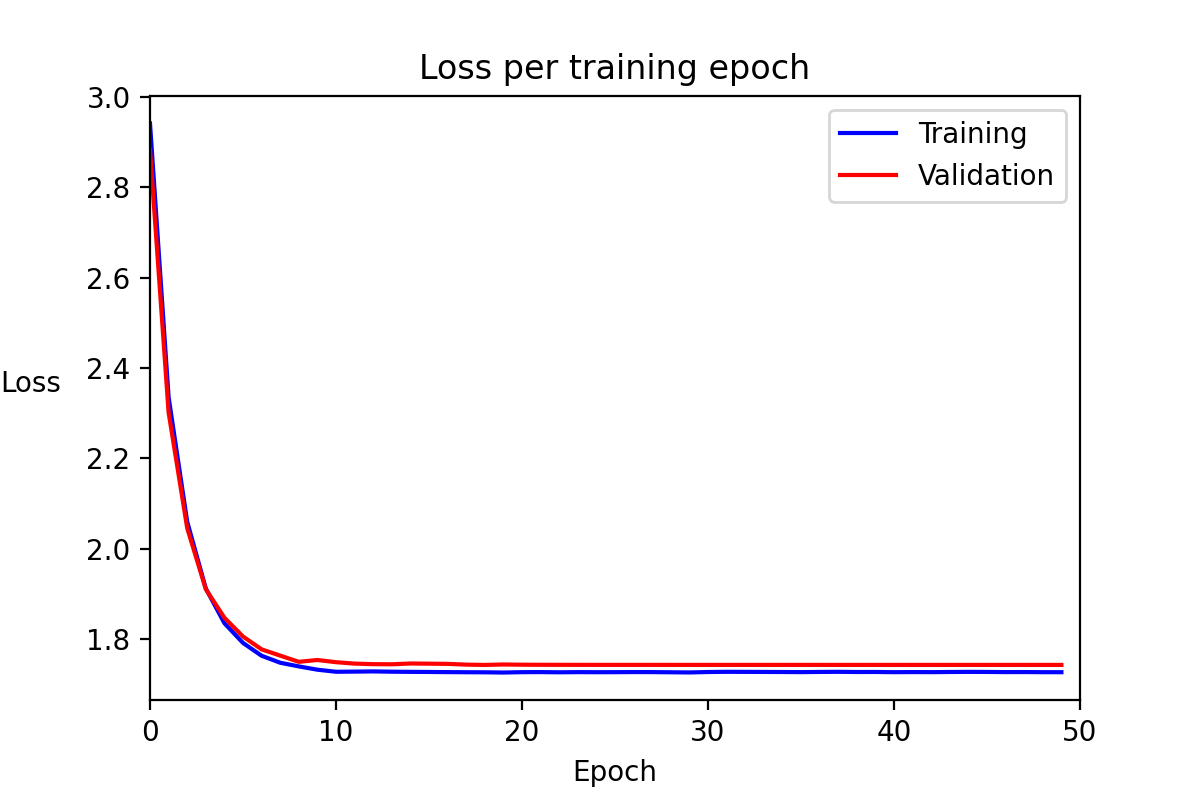
\includegraphics[width=7cm]{../plots/loss_v5.png}
		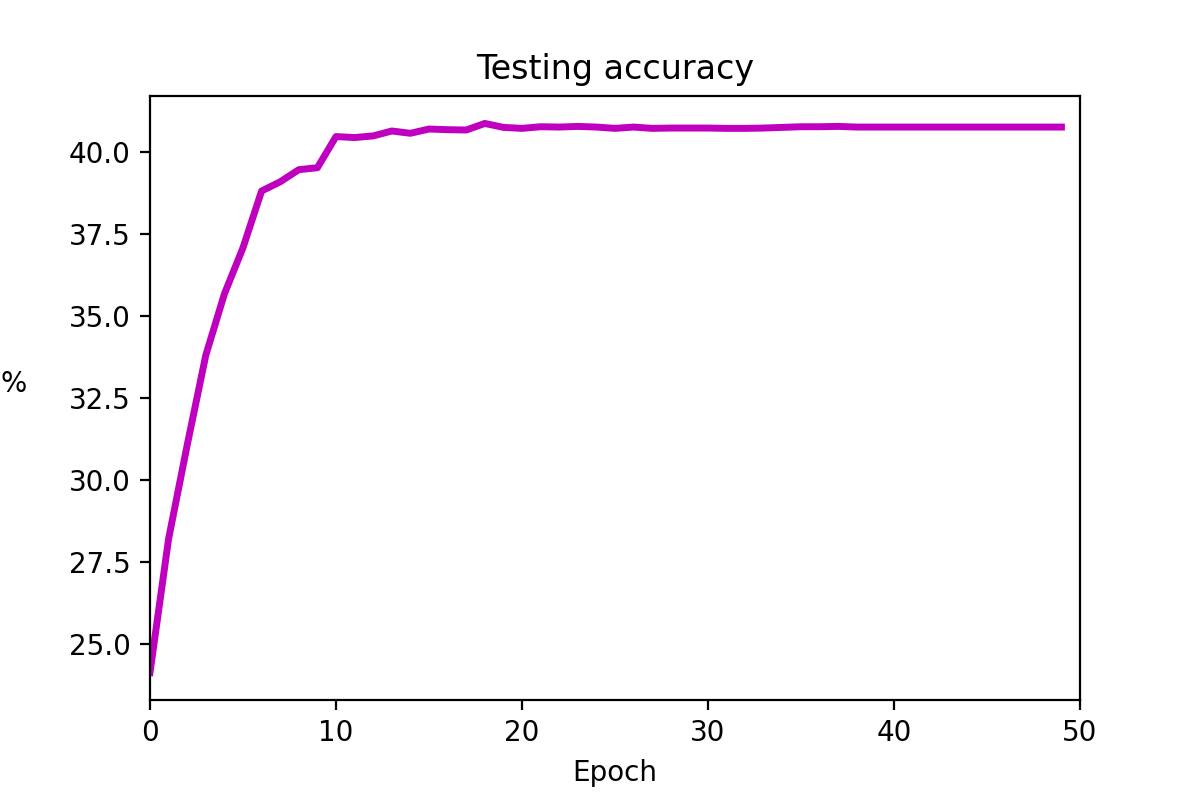
\includegraphics[width=7cm]{../plots/acc_v5.png}
		\caption{Loss and accuracy for optimal set of parameters}
		\vspace{0.2cm}
		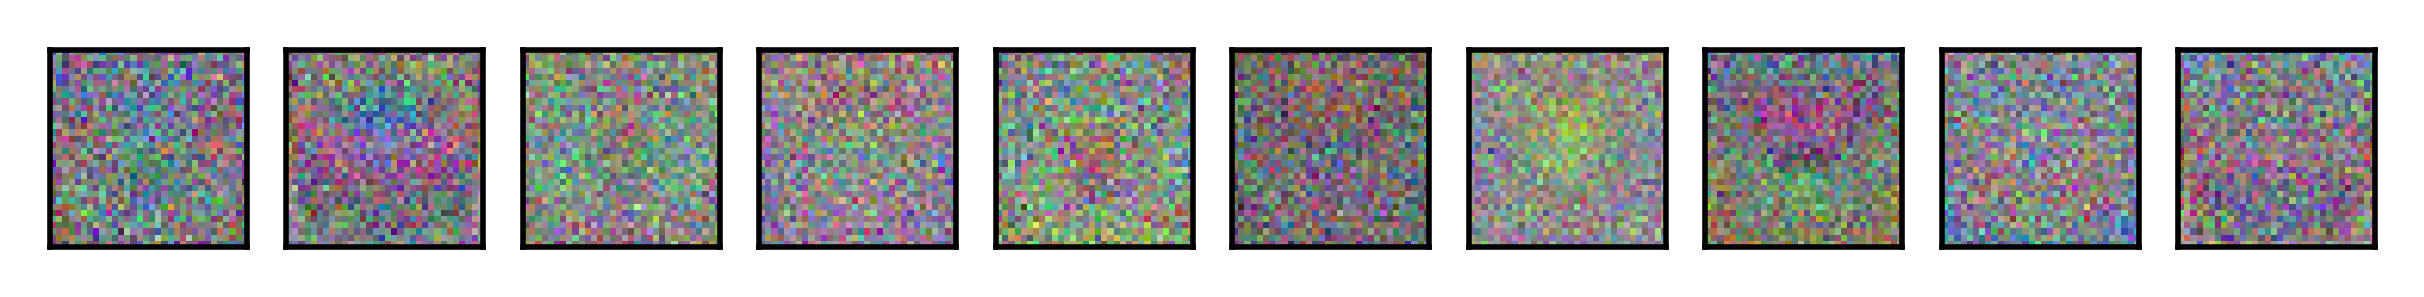
\includegraphics[width=12cm]{../plots/weights_v5.png}
		\caption{Class-specific weights for optimal set of parameters}
		%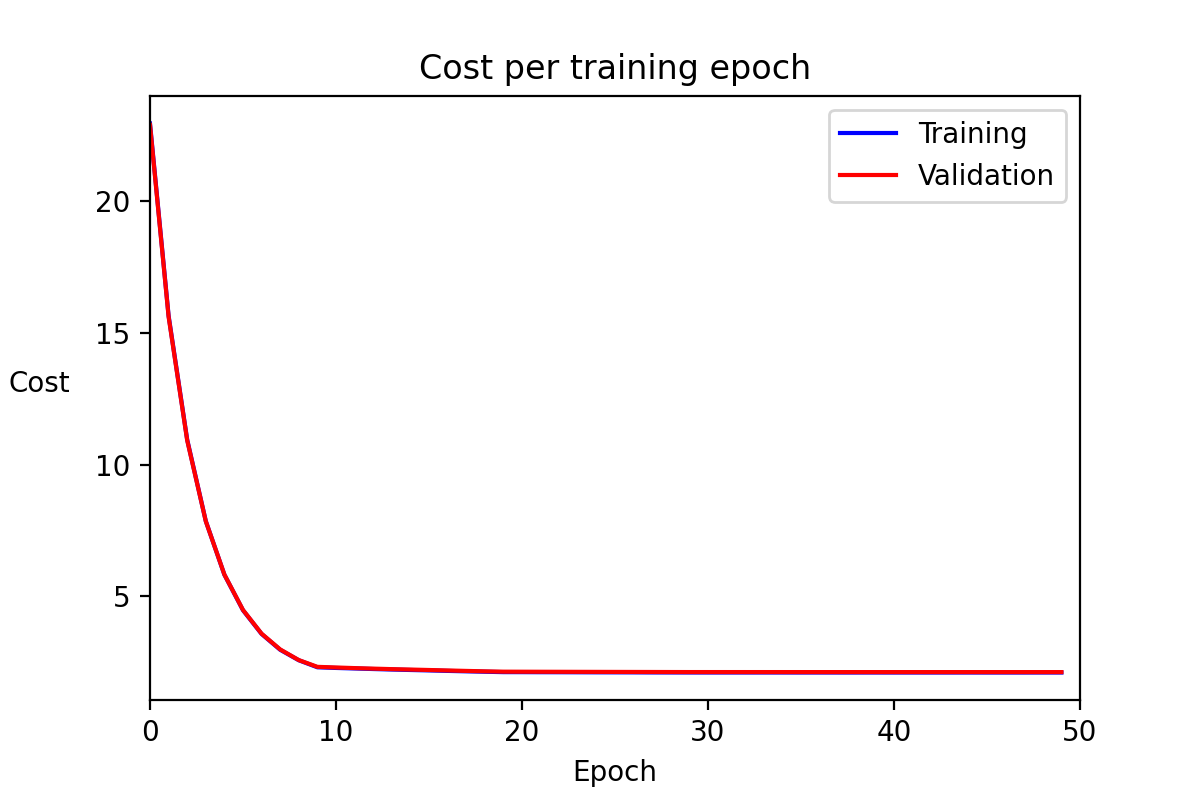
\includegraphics[width=7cm]{../plots/cost_v2.png}	
	\end{figure}


\newpage
\section*{Part II - Multiple Binary Cross-Entropy Losses}
\vspace{0.5cm}
\subsection*{Obtaining the gradient}
	In order to obtain the expression for $\partial\ell/\partial\bm{s}$, we consider the chain rule, where
	$$\dfrac{\partial\ell}{\partial\bm{s}} = \dfrac{\partial\ell}{\partial\bm{p}}\dfrac{\partial\bm{p}}{\partial\bm{s}}$$
	First, we considering differentiating the class-specific loss w.r.t. the correspoding probability, s.t. $\ell = -1/K \sum_{k=1}^K \ell_k$:
		$$\dfrac{\partial\ell_k}{\partial p_k} = \frac{\partial}{\partial p_k} \left[ (1 - y_k)\log(1 - p_k) + y_k \log(p_k)\right] = \frac{y_k - 1}{1 - p_k} + \frac{y_k}{p_k} $$
	Second, we recognize that $p_k = \sigma(s_k)$, wherer $\sigma: \mathbb{R} \rightarrow [0, 1]$ is the logistic sigmoid function, for which we also have that
	$$\sigma(s) = \frac{1}{1 + e^{-s}} = \frac{e^{s}}{e^{s} + 1}$$
	as well as $1 - \sigma(s) = \sigma(-s)$ and $\sigma'(s) = \sigma(s)(1 - \sigma(s))$. Hence, we get that
	\begin{align*}
		\dfrac{\partial \ell_k}{\partial s_k} &=  \frac{\partial}{\partial s_k} \left[ (1 - y_k)\log(1 - \sigma(s_k)) + y_k \log(\sigma(s_k))\right] \\
		&=\frac{y_k - 1}{1 - \sigma(s_k)}\sigma(s_k)(1 - \sigma(s_k)) + \frac{y_k}{\sigma(s_k)}\sigma(s_k)(1 - \sigma(s_k)) \\
		&=  (y_k - 1)\sigma(s_k) + y_k(1 - \sigma(s_k) \\
		&=  y_k - \sigma(s_k)  
	\end{align*}
	Hence, the Jacobians we're looking for are given by
	\begin{align*}
		\dfrac{\partial\ell}{\partial \bm{p}} &= -\frac{1}{K}\left[\bm{y}^T\text{diag}(\bm{p})^{-1} - (\bm{1} - \bm{y})^T \text{diag}(\bm{1} - \bm{p})^{-1}\right]\\
		\dfrac{\partial\bm{p}}{\partial \bm{s}} &= \text{diag}(\bm{p})\,\text{diag}(\bm{1} - \bm{p})
	\end{align*}
	such that
	\begin{align*}
		\dfrac{\partial\ell}{\partial \bm{s}} &= -\frac{1}{K}\left[\bm{y}^T\underbrace{\text{diag}(\bm{p})^{-1}\text{diag}(\bm{p})\,\text{diag}(\bm{1} - \bm{p})}_{=\text{diag}(\bm{1} - \bm{p})} -  (\bm{1} - \bm{y})^T \underbrace{\text{diag}(\bm{1} - \bm{p})^{-1}\text{diag}(\bm{p})\,\text{diag}(\bm{1} - \bm{p})}_{=\text{diag}(\bm{p})}  \right]\\
		&= -\frac{1}{K}\left[ \bm{y}^T\text{diag}(\bm{1} - \bm{p}) - (\bm{1} - \bm{y})^T\text{diag}(\bm{p})\right] \\
		&= -\frac{1}{K}\left[\bm{y} - \bm{y}^T\text{diag}(\bm{p}) - \bm{p} + \bm{y}^T\text{diag}(\bm{p}) \right] \\
		&= -\frac{1}{K}(\bm{y} - \bm{p})
	\end{align*}
	Hence, using the result from the previous loss, we should have that
	$$\dfrac{\partial\ell}{\partial \bm{W}} = -\frac{1}{K}(\bm{y} - \bm{p})\,\bm{x}^T, \quad \dfrac{\partial\ell}{\partial \bm{b}} = -\frac{1}{K}(\bm{y} - \bm{p})$$

\newpage
\subsection*{Results}
	I implemented the linear classifier with a \texttt{sigmoid} activation and the multiple binary cross-entropy loss for a number of parameter settings. The loss, accuracy and class-specific weights have been plotted on the following page. Due to the $1/K$ factor in the loss, I have used a slightly higher learning rate for this part, $\eta=0.01$ or $\eta=0.05$, with a slightly modified decay rate, e.g. reducing the learning rate by half every $10$ steps. Overall, the results are comparable to those when using the \texttt{softmax} activation, but the achieved accuracy is actually lower across all tests compared to the highest accuracy achieved with the \texttt{softmax}. However, it does seem that similarly to using the \texttt{softmax}, the highest accuracy is achieved when using a moderate regularization parameter - again, in this case $\lambda = 0.1$. In fact, the performance is somewhat worse when using $\lambda = 1.0$ as compared to using $\lambda = 0.0$.\\\\
%
In order to compare the \texttt{softmax} and \texttt{sigmoid} activations, I trained two separate models with the optimal set of parameters found for each type. The class-specific prediction results and the parameter setting are shown in the plots and table below. The results are in fact very similar. Both models achieve a relatively low accuracy for the category $2$ and $3$, while they both achieve a relatively high accuracy for cateogories $0$, $1$, and $6$. The \texttt{softmax} model also seems to achieve a slightly better result for category $7$. The differences, however, are marginal. I wouldn't call this overfitting, since the class-specific accuracies are fairly well-distributed across the classes, with the exception of $2$ to $4$ - for which both models fail. 

	\begin{figure}[h!]
		\centering
		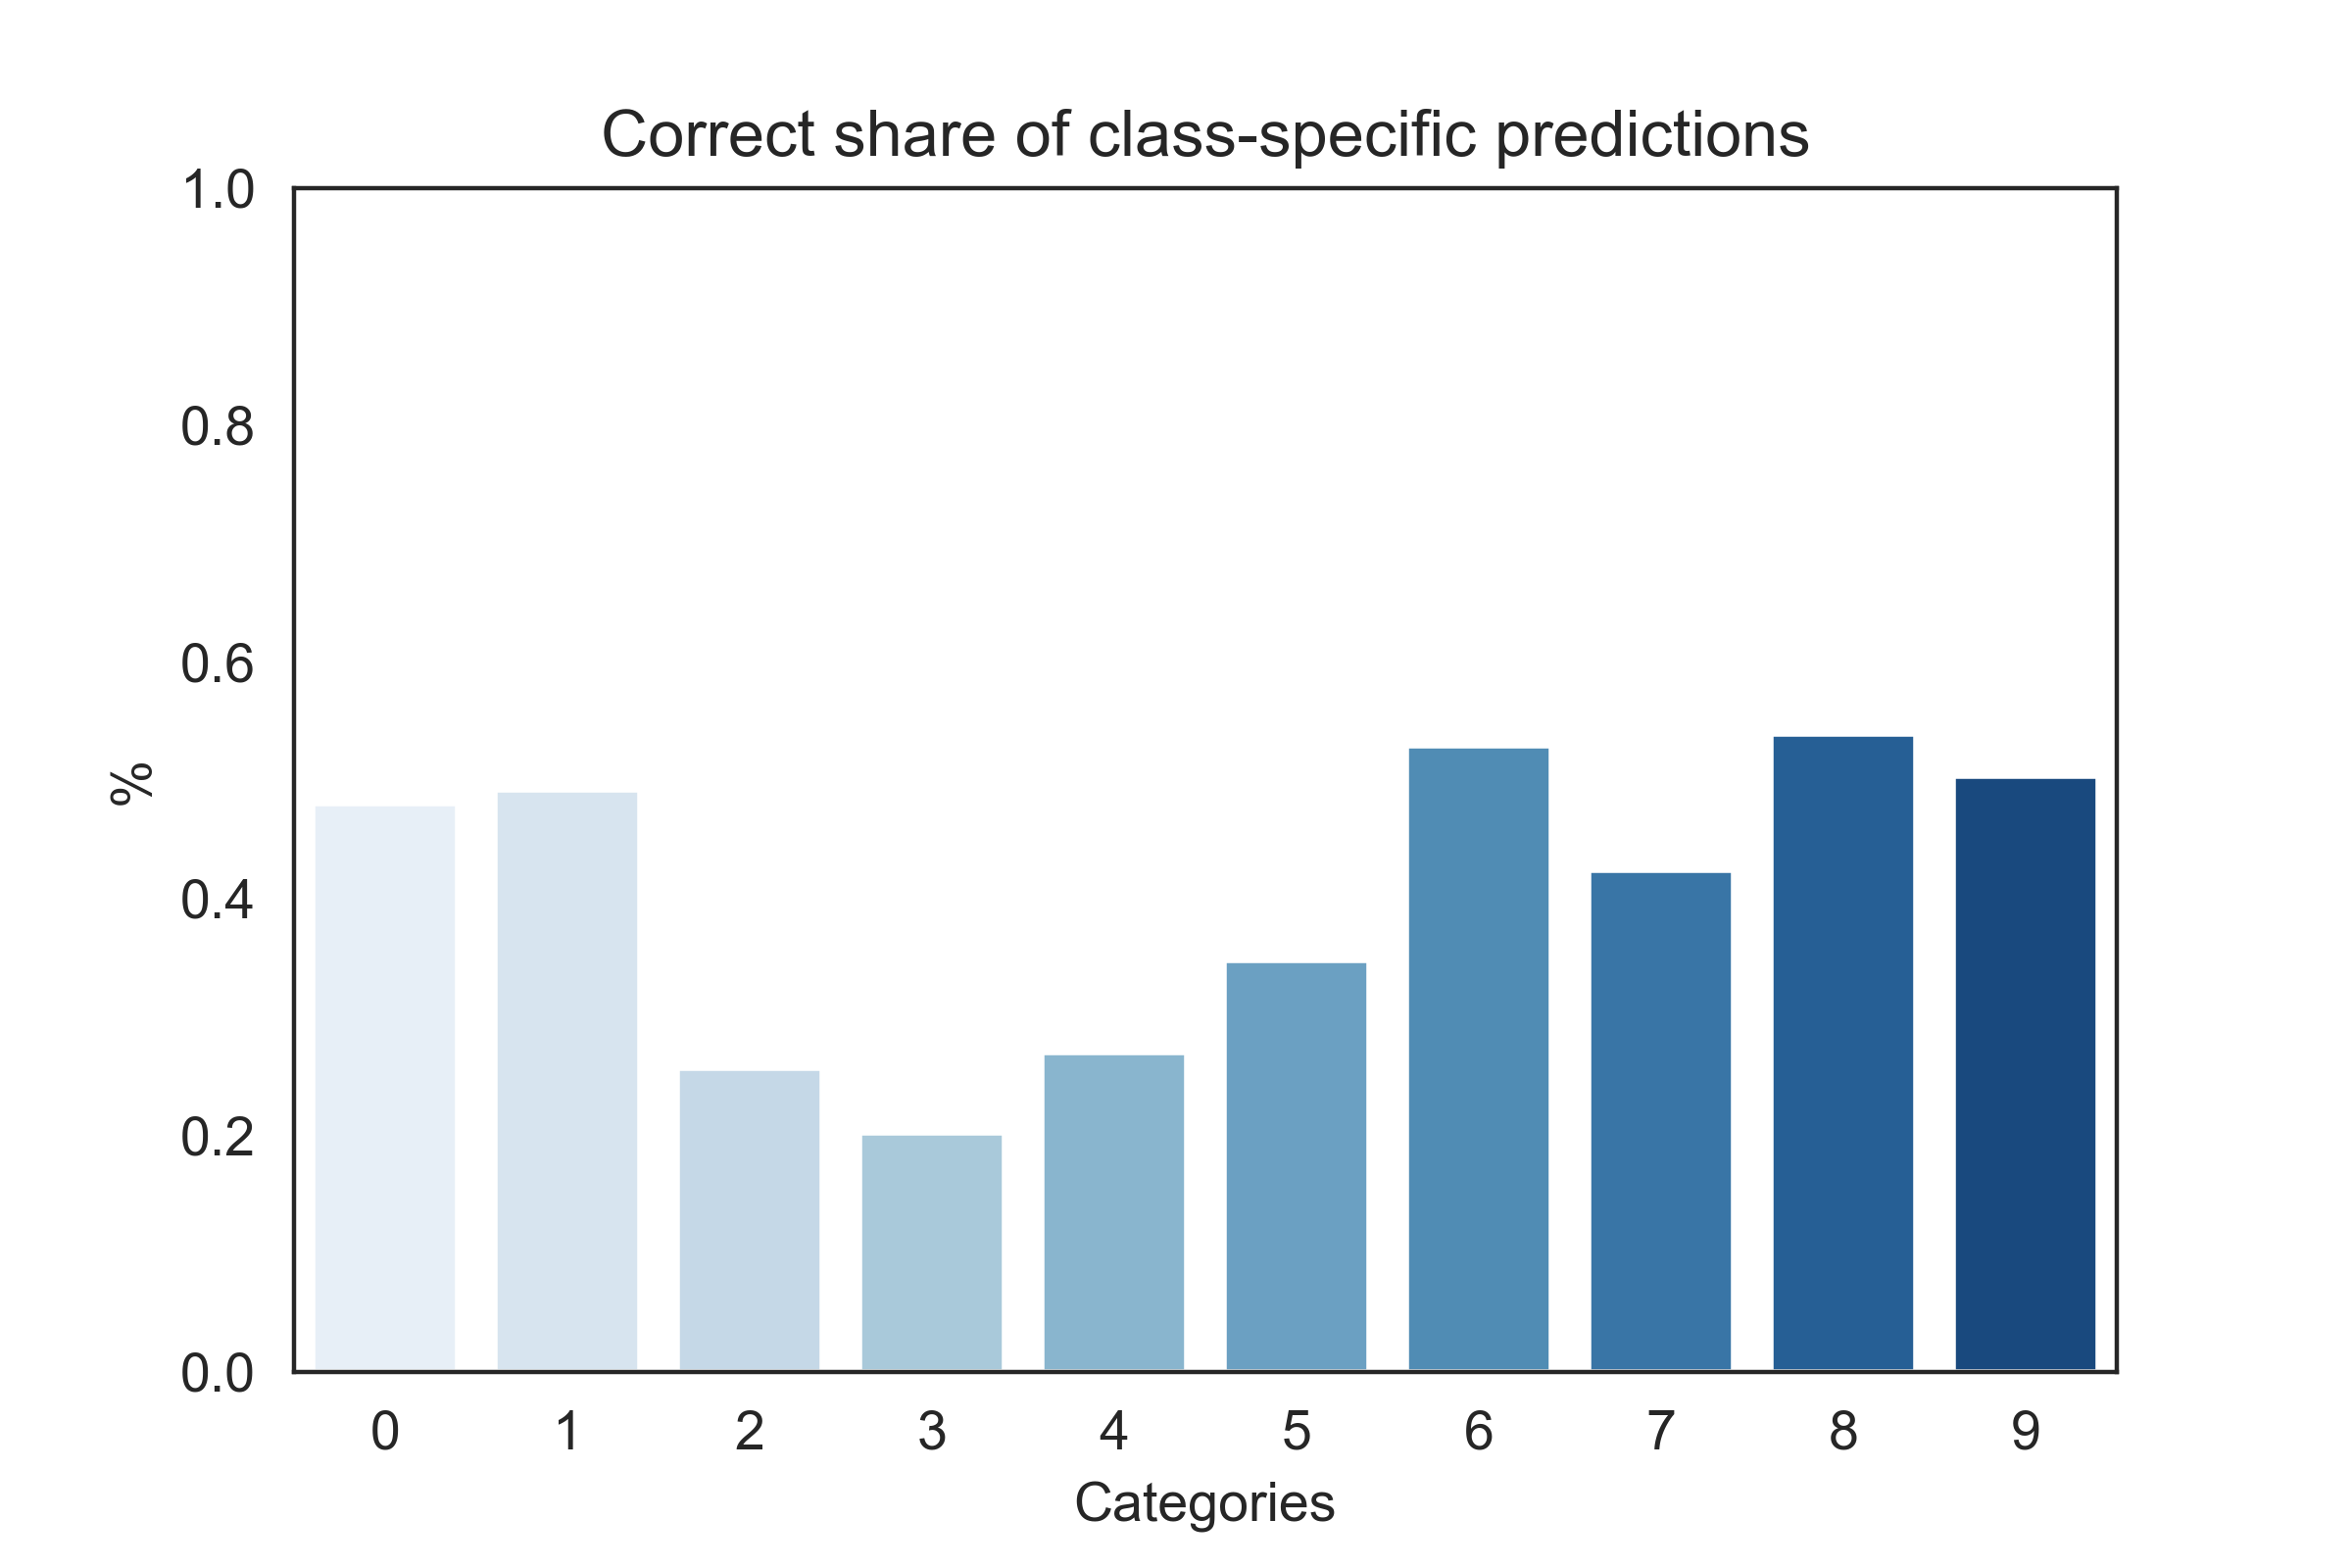
\includegraphics[width=7cm]{../plots/softmaxPreds.png}
		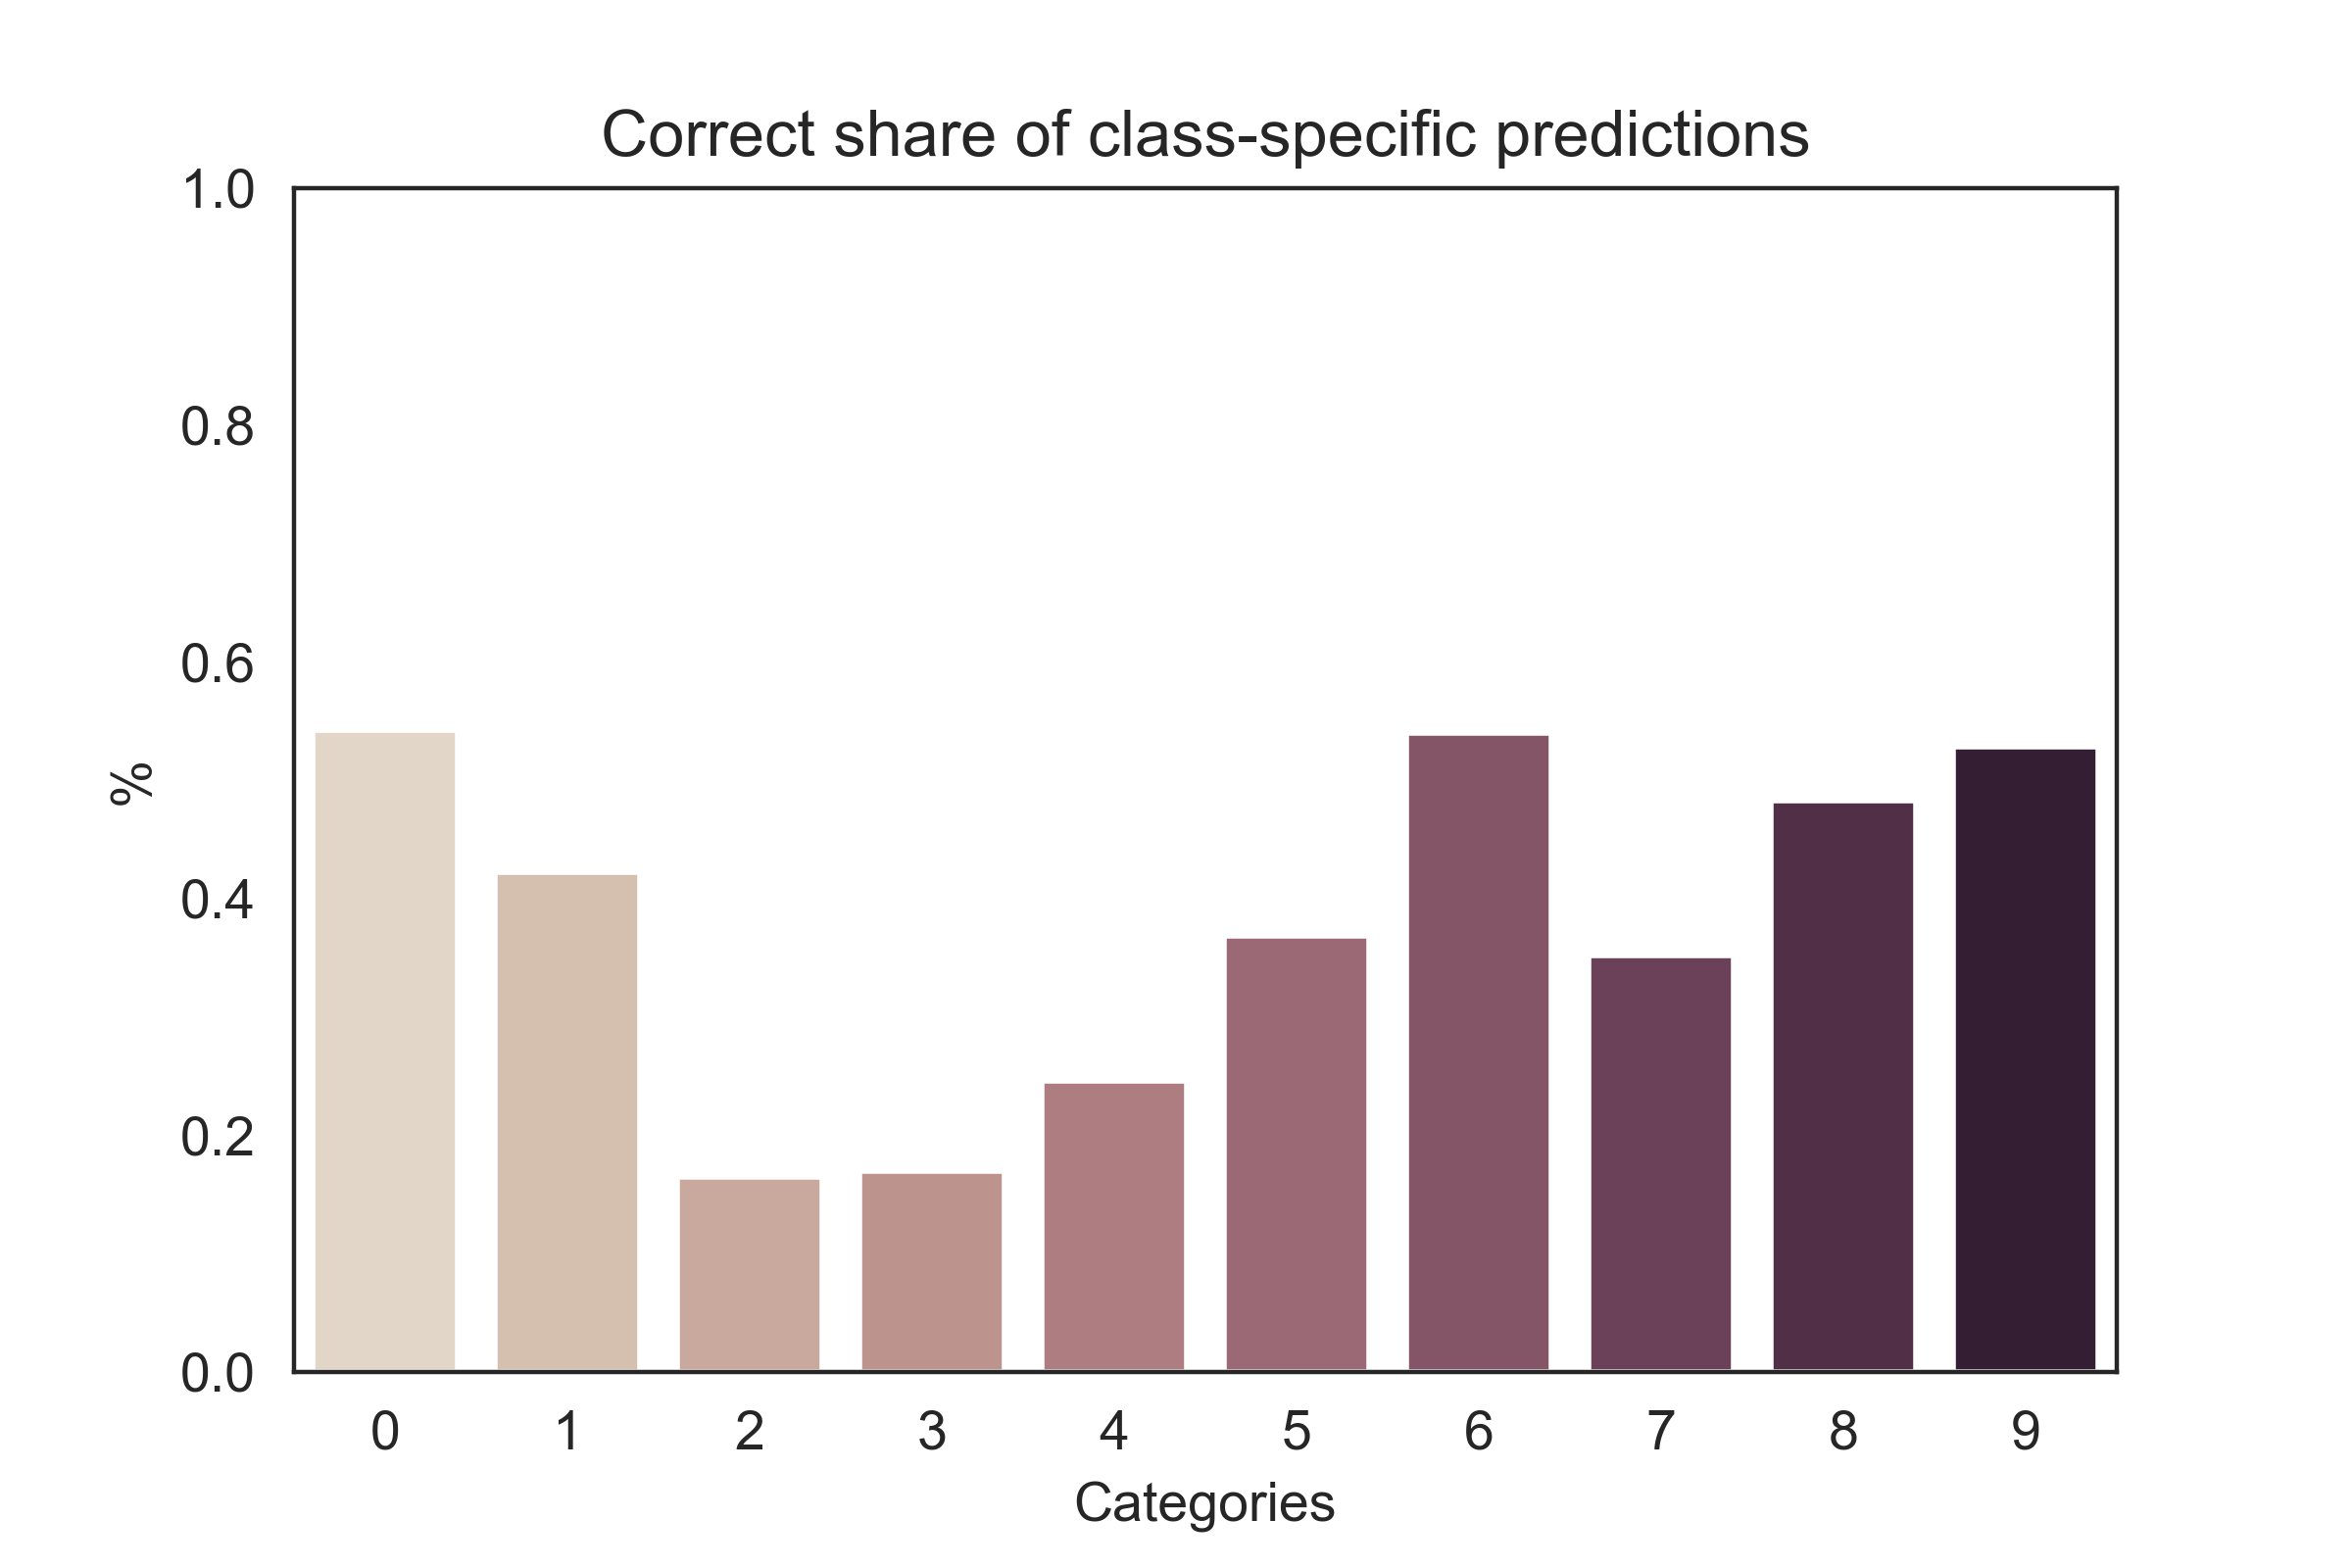
\includegraphics[width=7cm]{../plots/sigmoidPreds.png}
		\caption{Class-specific accuracy for \texttt{softmax} (left) and \texttt{sigmoid} (right)}
	\end{figure}
	\begin{center}
		\begin{tabular}{|l||l|l|l|l|l|c|}
			\hline
			Activation & \texttt{batchN} & \texttt{epochsN} & $\eta$ & $\eta_n$ & $\lambda$ & $P_{flip}$ \\ \hline
			\texttt{softmax} & 100 & 50 & 0.01 & 10 & 0.1 & 0.2 \\
			\texttt{sigmoid} & 50 & 50 & 0.01 & 0 & 0.1 & 0.5\\\hline
		\end{tabular}
	\end{center}

\newpage
	\begin{figure}[h!]
		\centering
		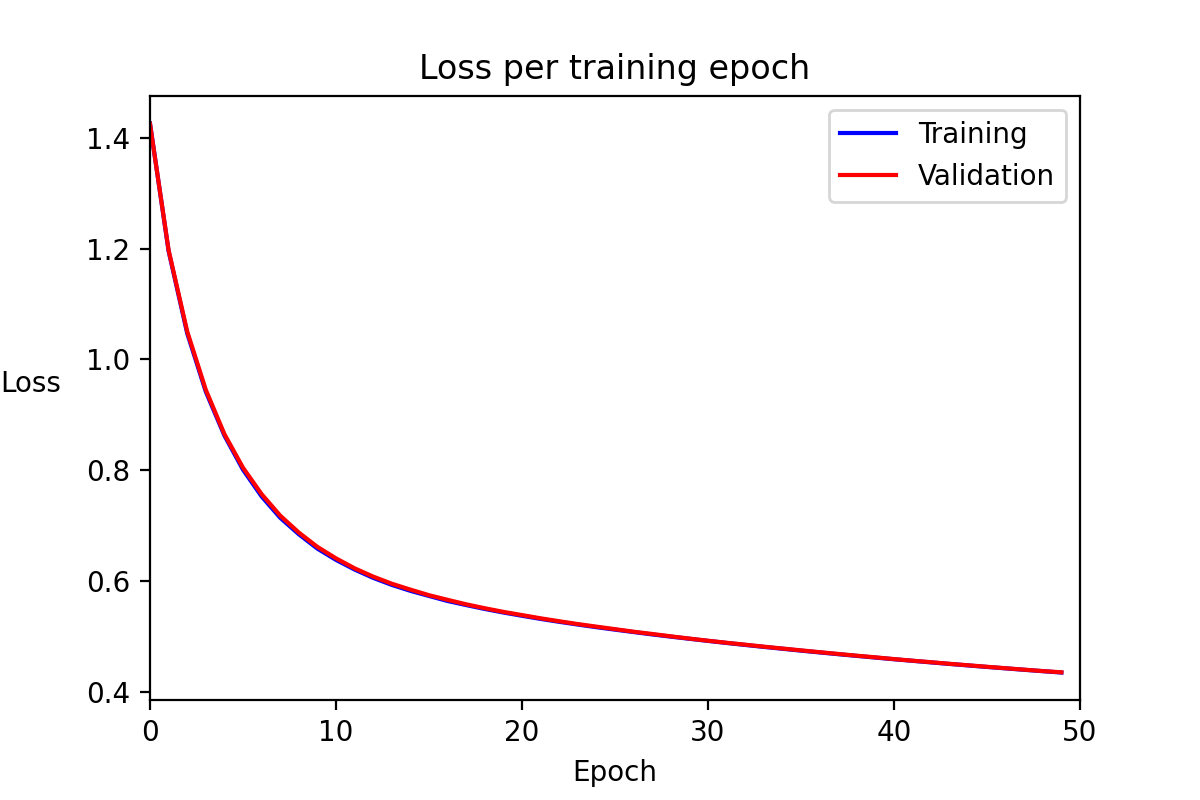
\includegraphics[width=7cm]{../plots/loss_v9.png}
		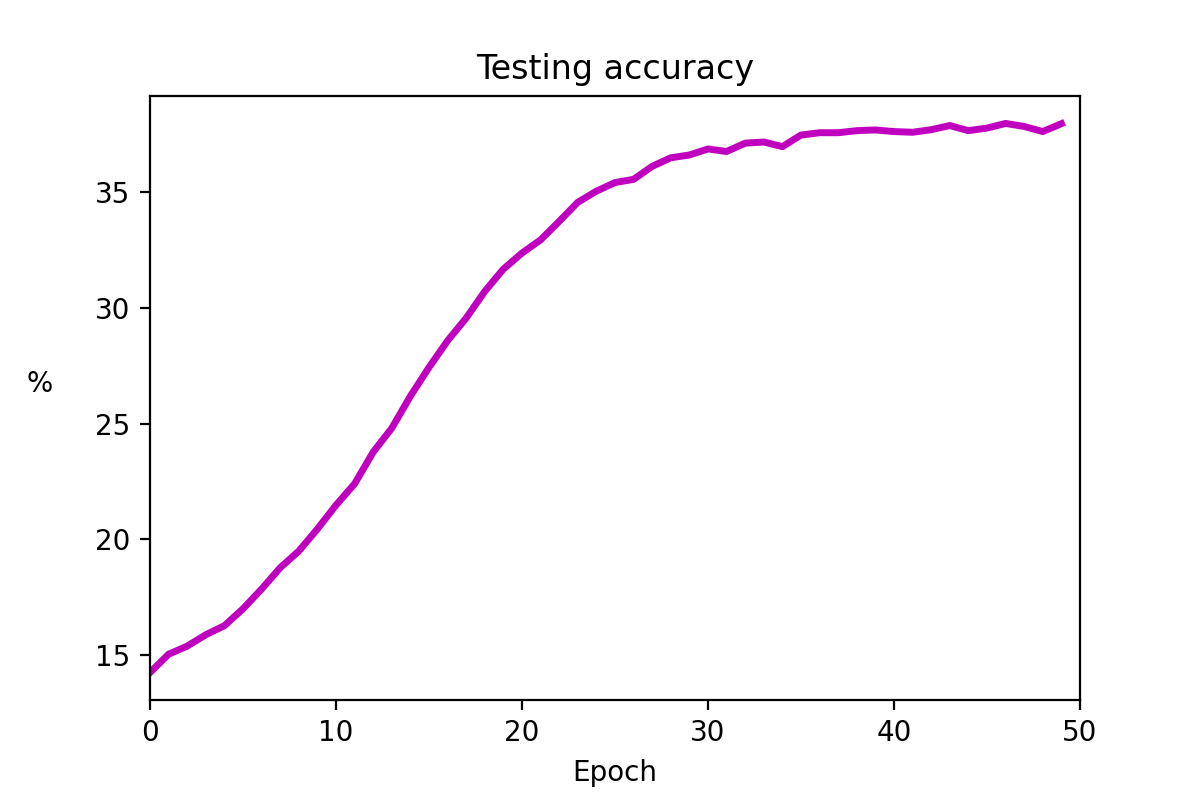
\includegraphics[width=7cm]{../plots/acc_v9.png}
		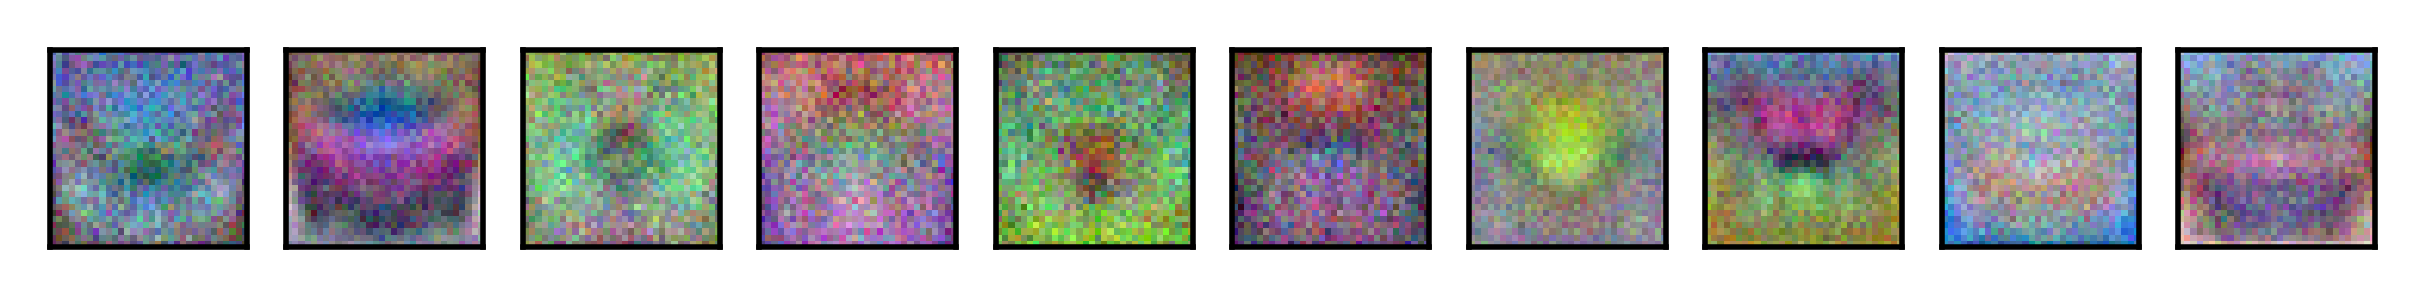
\includegraphics[width=12cm]{../plots/weights_v9.png}
		\caption{\texttt{sigmoid} with $\lambda=0.1$, $\eta=0.01$, \texttt{batchN} $=100$, \texttt{epochsN} $=50$, $P_{\text{flip}}=0.5$}
		\vspace{0.2cm}
		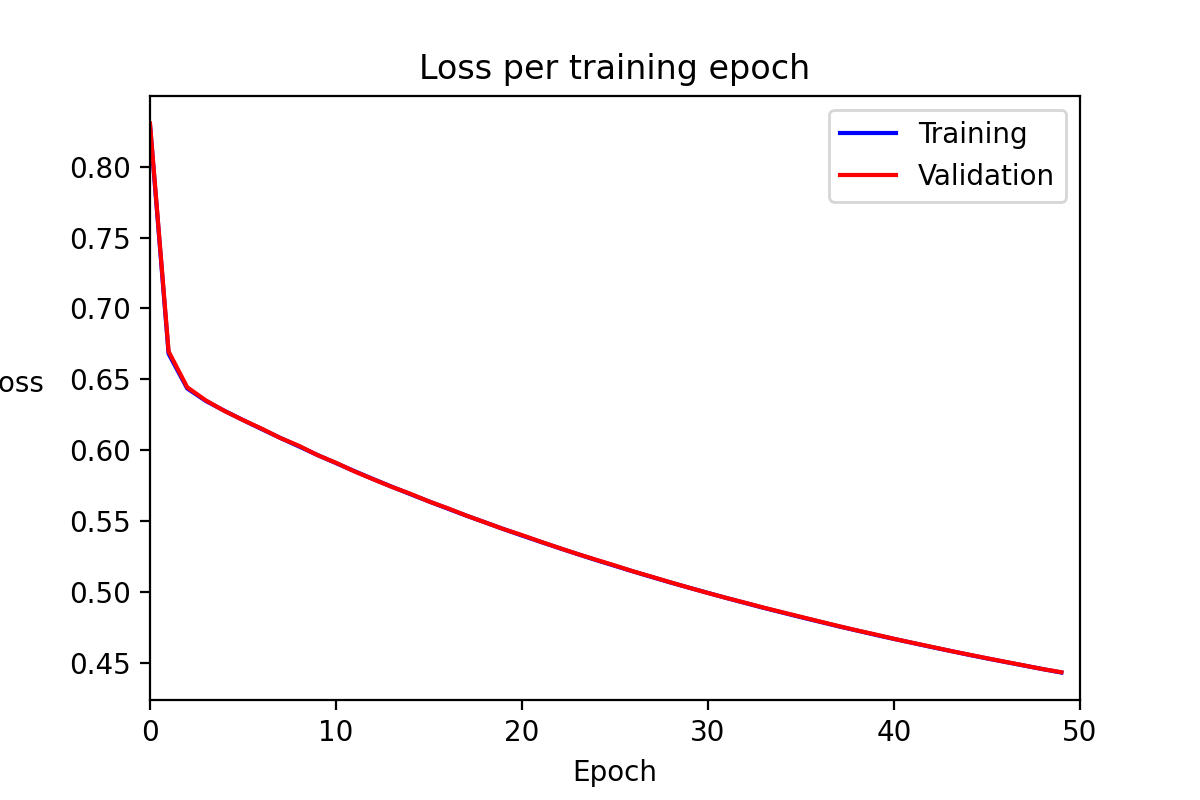
\includegraphics[width=7cm]{../plots/loss_v10.png}
		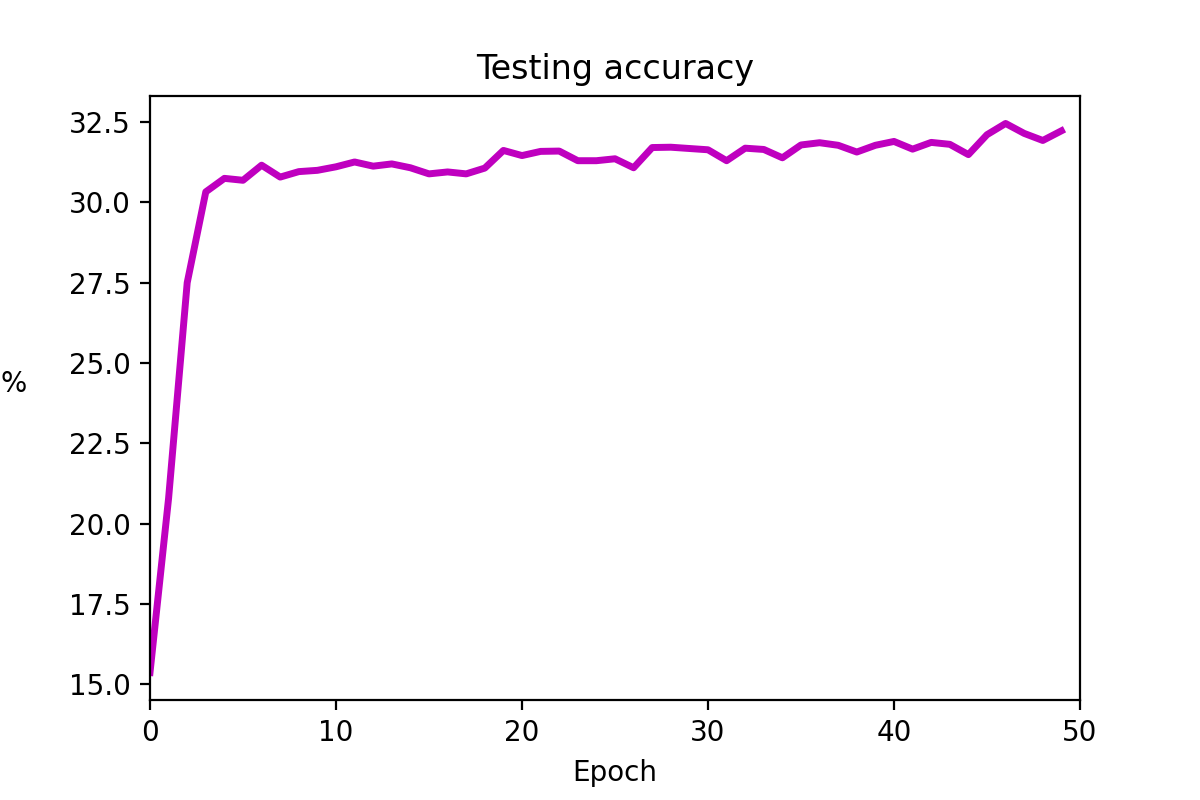
\includegraphics[width=7cm]{../plots/acc_v10.png}
		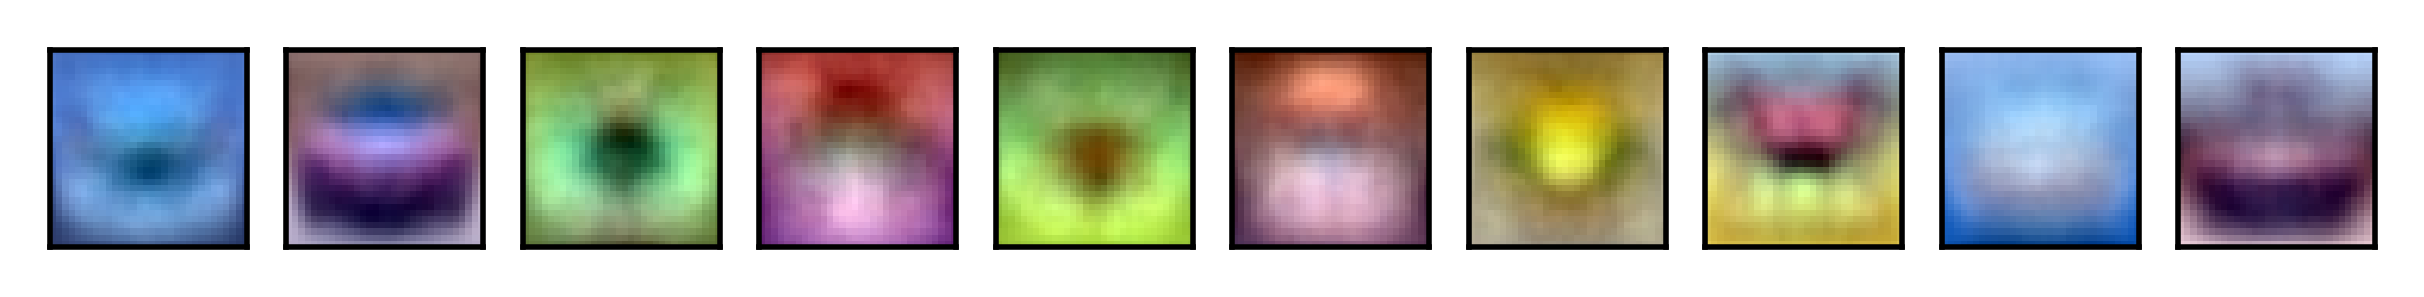
\includegraphics[width=12cm]{../plots/weights_v10.png}
		\caption{\texttt{sigmoid} with $\lambda=1.0$, $\eta=0.01$, \texttt{batchN} $=100$, \texttt{epochsN} $=50$, $P_{\text{flip}}=0.5$}
		\vspace{0.2cm}
		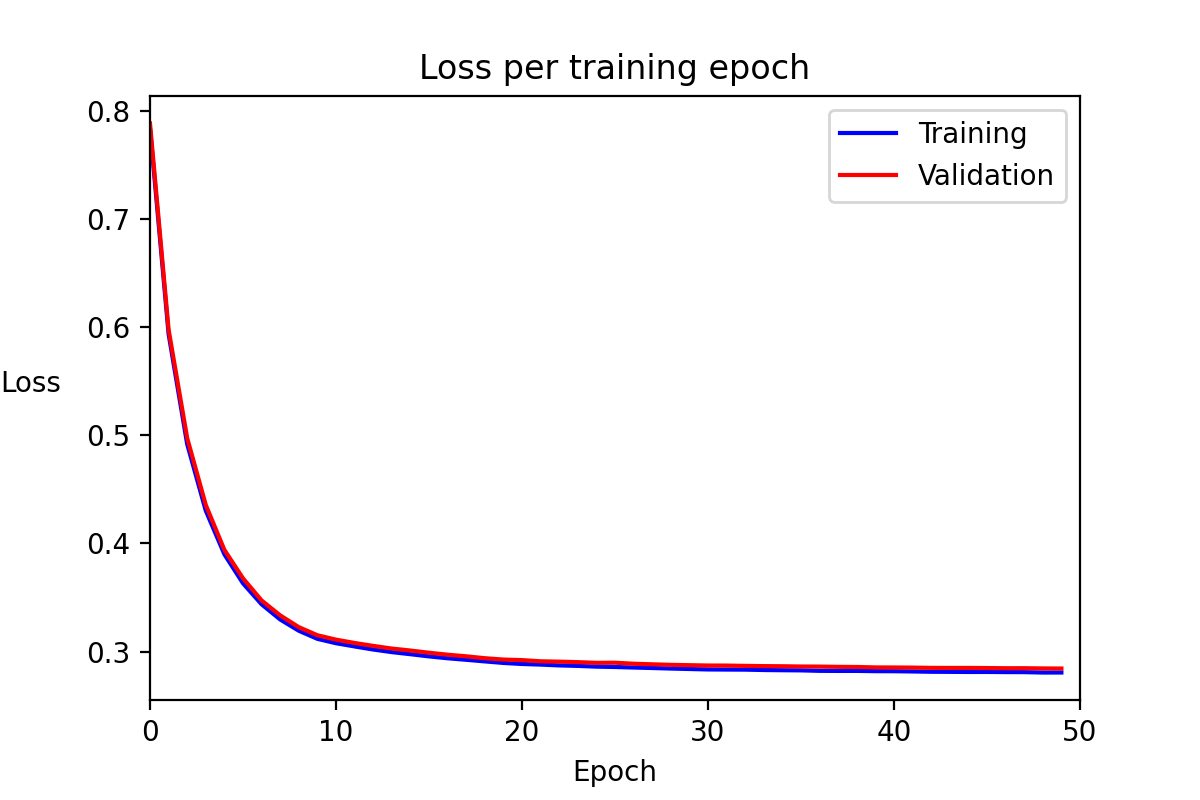
\includegraphics[width=7cm]{../plots/loss_v11.png}
		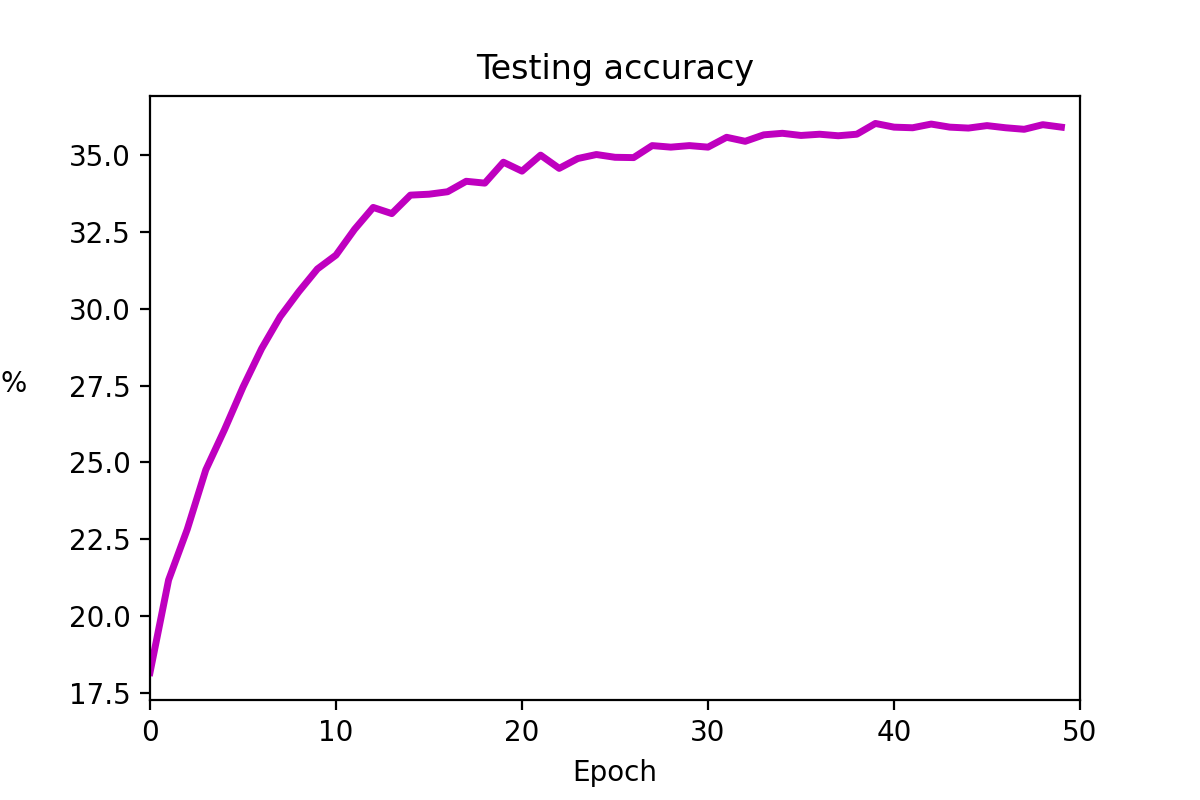
\includegraphics[width=7cm]{../plots/acc_v11.png}
		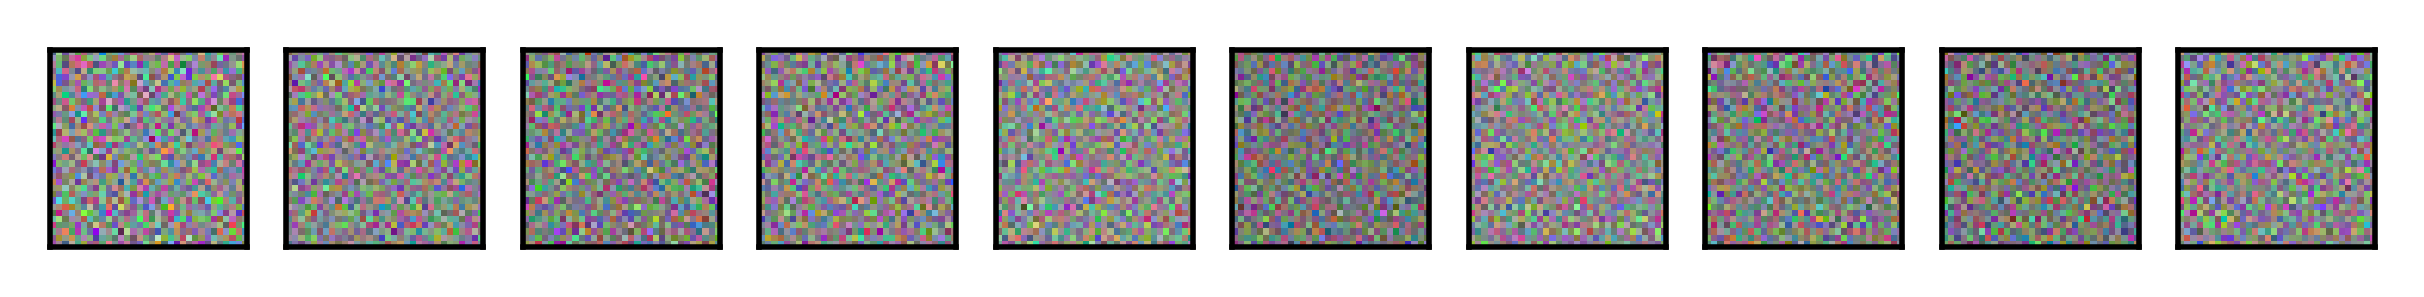
\includegraphics[width=12cm]{../plots/weights_v11.png}
		\caption{\texttt{sigmoid} with $\lambda=0.0$, $\eta=0.01$, \texttt{batchN} $=100$, \texttt{epochsN} $=50$, $P_{\text{flip}}=0.1$}
		%\vspace{0.2cm}
	\end{figure}

\end{document}